%Original version in April 2002 by Antje Endemann
%
%Adapted for usage in Student Conference course by jubo (050118).
%Optimized for usage with pdflatex. For usage with plain latex,
%figures must be in Postscript (.ps or .eps files) and additional
%packages must be imported.
%Last updated 100105 by jubo
%
%This template works for outline and annotated bibliography
%(deliverable 2) without any changes.
%For usage with full and final papers (deliverables 3 and 4a/b)
%you must make several changes. All necessary changes are
%described in three specific commented sections preceded by
%`%%%%% BEGIN OF ADJUSTMENTS SECTION %%%%%'.
%The changes are in order of appearance:
%   - adjust the `\documentclass' command
%   - uncomment the abstract section
%   - adjust the `\bibliographystyle' command

%%%%% BEGIN OF 1st ADJUSTMENTS SECTION %%%%%
% You must use only one of the following `\documentclass' commands
% For the outline and annotated bibliography (deliverable 2)
% you must use the following command:
%
\documentclass[runningheads,a4paper,oribibl]{llncs}
%
%For the full and final paper (deliverables 3 and 4a/b)
% you must use the command below (and put the one above in comments).
% In other words, the 'oribib' option must be used for Deliverable 2
% but not for 3 and 4a/b.
% 
%
%\documentclass[runningheads,a4paper]{llncs}
%
%%%%% END OF 1st ADJUSTMENTS SECTION %%%%%

\usepackage[T1]{fontenc}  %% needed for special characters (umlaut)
\usepackage[latin1]{inputenc}
\usepackage{graphicx}     %% for graphical things such as including pictures
\usepackage{url}          %% for proper formatting of URLs

\begin{document}

\pagestyle{headings}

\mainmatter

\title{Typesetting Your Outline, Annotated Bibliography, and Full Paper for the Course Student Conference in Computing Science\thanks{based on an earlier version by J�rgen B�rstler}}

% The abbreviated title will be shown in the headers of even pages.
% You should use the full title unless it is too long.
\titlerunning{Example Outline and Annotated Bibliography}

\author{Frank Drewes}

\institute{
    Department of Computing Science \\
    Ume� University, Sweden \\
    \email{drewes@cs.umu.se}
}

\maketitle

%%%%% BEGIN OF 2nd ADJUSTMENTS SECTION %%%%%
% Do NOT include an abstract in the outline and annotated bibliography
% (deliverable 2). For the full and final paper (deliverables 3 and 4a/b),
% you must uncomment the following two commands and place your text for
% the abstract in between them.
%
% \begin{abstract}
%   Here goes the actual text of your abstract.
% \end{abstract}
%
%%%%% END OF 2nd ADJUSTMENTS SECTION %%%%%


\section{Introduction}
An outline is a draft of a research paper. It will help you to organize
your thoughts, ideas and materials in a logical form.
It should be detailed enough to make the following clear to yourself and
to the reader.
\begin{description}
   \item[Purpose] What exactly is (will be) the goal of your paper.
         You should therefore develop some kind of \emph{thesis statement},
         i.e., a specific statement, research question or hypothesis you
         want to answer or investigate in more detail.
   \item[Rationale/Motivation] Make clear why your thesis
         statement is interesting or important. A general motivation like
         ``I want to learn more about topic X'' definitely is not good enough.
   \item[Contents] What your final paper approximately will contain.
   \item[Resources] The resources you intend to use in your work. This
         will be specified in more detail in the annotated bibliography
         (reference section).
\end{description}

The main sections and subsections should be drafted and contain some
actual text or information about the planned contents, like the
following.
\begin{itemize}
  \item Meaningful section and subsection headers.
  \item Some (preliminary) text in all or most of the sections and subsections
        that help you organize your thoughts, ideas and materials. This will
        also give the reader (and yourself) a feeling for the planned contents.
  \item Citations of literature you intend to use to support your reasoning,
        like~\cite{beck:1989} or~\cite{booch:1999,fleury:2000,thimbleby:1999}.
  \item Drafts of figures (see Figure~\ref{fig:UML} and Figure~\ref{fig:picture}),
        tables (see Table~\ref{tab:table}), or examples.
\end{itemize}


\section{Annotated Bibliography}\label{sec:bibl}
The annotated bibliography is a list of literature references, where each
reference is followed by an ``annotation''. Please do not confuse this
annotation with an abstract. An annotation should describe and comment
the reference \emph{in your own words}, and it should focus on the aspects that
are \emph{important to you}.

The actual data of the annotated bibliography is stored in a separate text file, a
BIBTeX database such as the file \texttt{demo.bib}. Each entry describes a reference
and consists of a number of fields recording title, author, etc. Annotations
and other information can be stored in additional fields. Please note that you do
not need to delete any annotations from your BIBTeX file for later deliverables.
The annotations will be disregarded by BIBTeX because you will use a different
BIBTeX formatting style for the references in Deliverables~3 and~4a/b
(see the commented section at the end of \texttt{demo.bib}).


\section{Formatting Guidelines}
Please check the lecture overheads and the submission guidelines for
details on formatting and other requirements. The outline should consist of
about two pages plus the annotated bibliography.


\section{Subsections, Lists, Tables, and Figures}
Sections and subsections on the first and second levels
are numbered automatically. Subsections on levels three or more do not get
section numbers in the formatting style we use here.


\subsection{Lists}
Lists can be itemized, like in the list right before Section~\ref{sec:bibl},
or enumerated as below. Of course, lists can be nested.

\begin{enumerate}
  \item This is an example of a nested enumerated (numbered) list.
  \begin{enumerate}
     \item First subitem.
     \item Second subitem.
  \end{enumerate}
  \item Second item.
  \item And so on.
\end{enumerate}


\subsection{Tables}
Tables are constructed using the \texttt{tabular}
environment. For an example, please check the \LaTeX\ source code for
Table~\ref{tab:table}.
%
\begin{table}
   \centering
   \begin{tabular}{|l|p{2,8cm}|c|r|}
     \hline
     \textbf{left aligned} & \textbf{formatted as a paragraph} &
       \textbf{center aligned} & \textbf{right aligned}\\
     \hline
     row 2 &
       it is possible to have long texts in tables if they are
       formatted as a paragraph &
       this does not work well otherwise & 123\\
     row 3 & 45 & 6 & 7\\
     \hline
   \end{tabular}
   \caption{A simple table with 4 columns and 3 rows.\label{tab:table}}
\end{table}%
%
There are several useful extensions of the \texttt{tabular} environment. One of them
is \texttt{tabularx}, which lets you explicitly define the table width (normally
\texttt{\string\linewidth}) and has a column type \texttt X whose width is automatically calculated
from this. If you want to use it, load the package \texttt{tabularx} and have a look
at its documentation.

\subsection{Floating Tables and Figures}
Tables and figures should normally be put into the environments \texttt{table}
and \texttt{figure}, respectively. In this way, \LaTeX\ will automatically
attempt to move the table or figure to a place where it fits. Moreover, you can
(and should) give an informative caption and define a
symbolic label used to refer to them from the text. The labelling mechanism works
as follows. In or after the caption of the float, you place a the command
\texttt{\string\label\{my label\}}. Now \LaTeX\ will produce the numer of that
float in all places where you use the command \texttt{\string\ref\{my label\}}.
You can also refer to the page number on which the float appears by using the
command \texttt{\string\pageref\{my label\}}. For example, in the caption of
Table~\ref{tab:table} the command \texttt{\string\label\{tab:table\}} was used,
so that this sentence could refer to it by \texttt{Table\raisebox{-.5ex}{\string~}\string\ref\{tab:table\}}.
Note that a tilde is used instead of a space character between the word Table and the
referencing command. This creates a nonbreaking space, which prevents \LaTeX\ from
inserting a line break between the two. The probably obvious purpose is to avoid ugly linebreaks
such as Table \ref{tab:table}.\footnote{The same kind of nonbreaking space should be used in front of
\texttt{\string\pageref} and \texttt{\string\cite}, for the same reasons.}

The contents of a
``float'' can be any \LaTeX\ material, but tables often consist of \texttt{tabular}
material and figures often contain graphics imported via the command
\texttt{\string\includegraphics}.

In plain \LaTeX\ (\textit{latex}), imported graphics must be in \textit{PS/EPS} format.
If you use \textit{pdflatex}, which we strongly recommend,
you can include a range of different formats, like for example \textit{PDF}
(see Figure~\ref{fig:UML}) or \textit{JPG} (see Figure~\ref{fig:picture}).

\begin{figure}
   \centering
   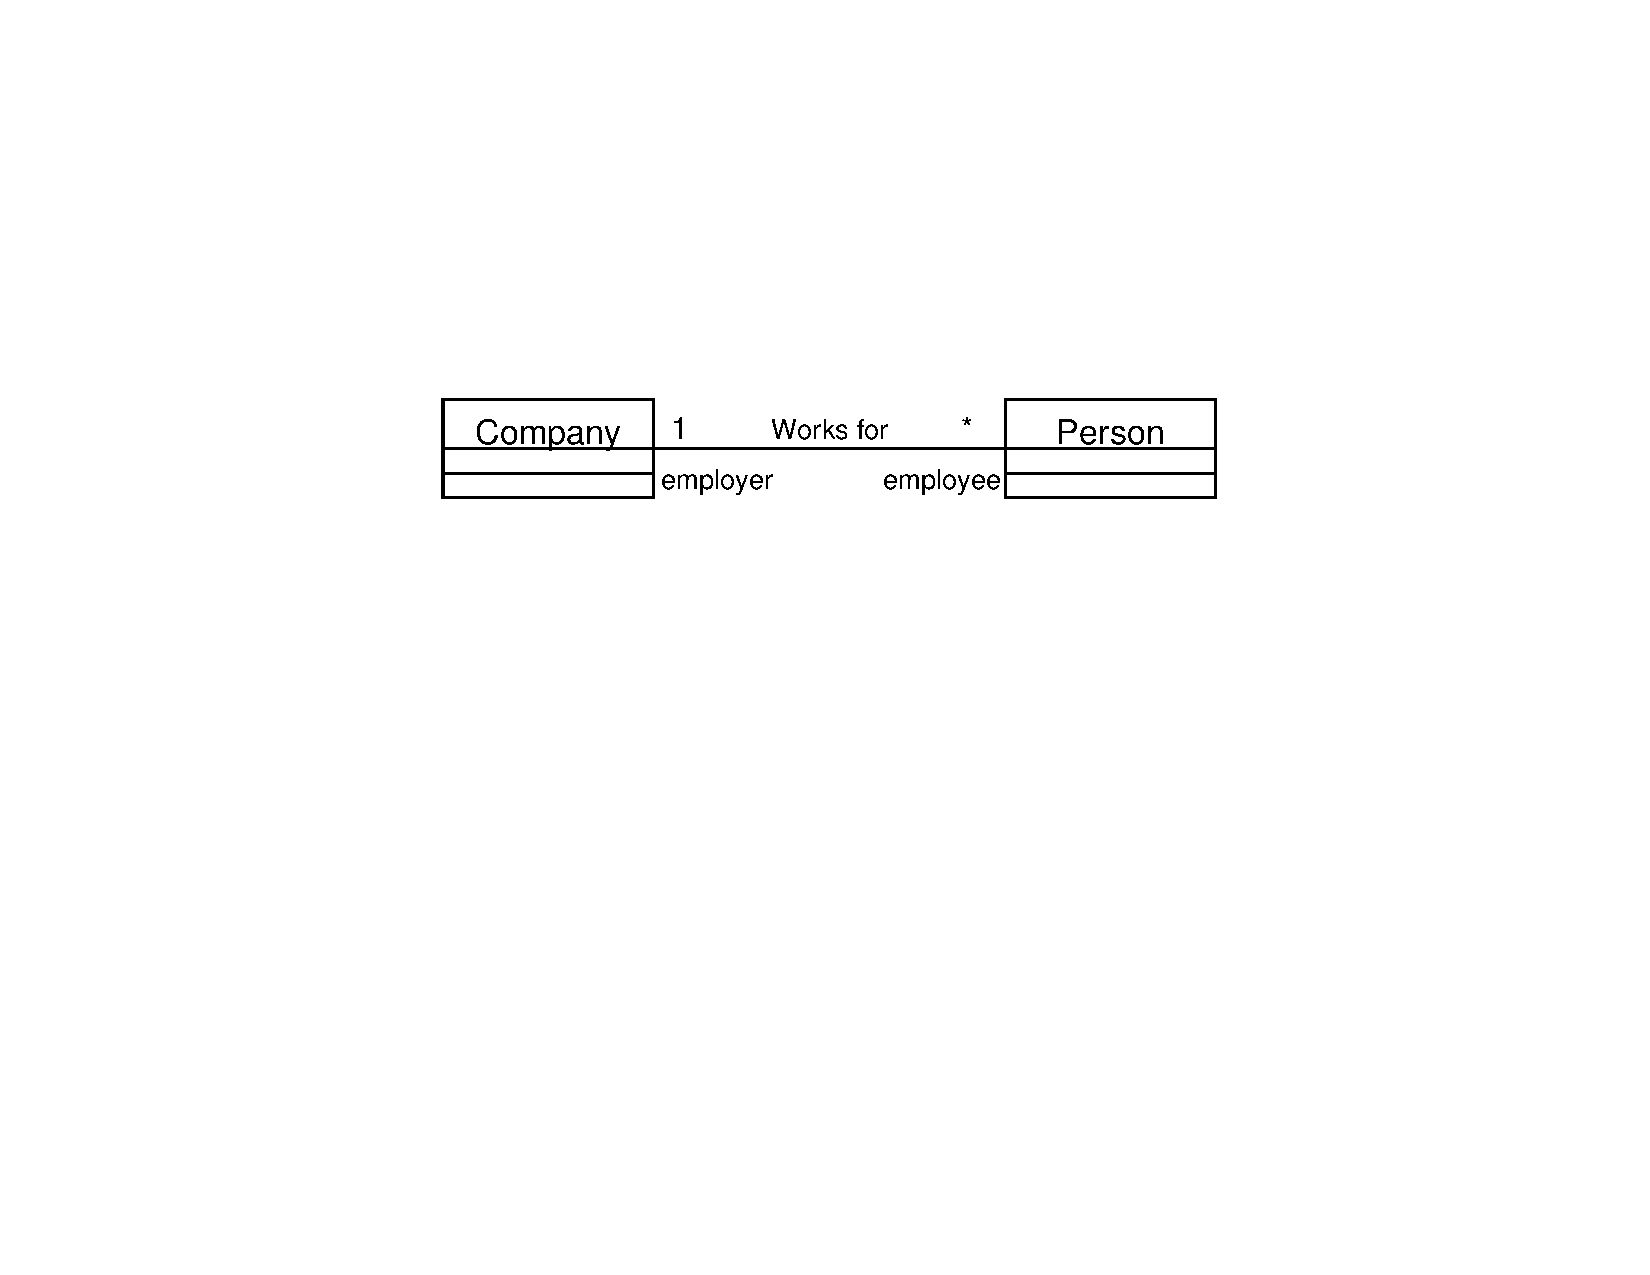
\includegraphics[width=0.75\textwidth]{UMLdiagram}
   \caption{A figure from a PDF file (must be PDF 1.4 compatible).\label{fig:UML}}
\end{figure}

\begin{figure}
   \centering
   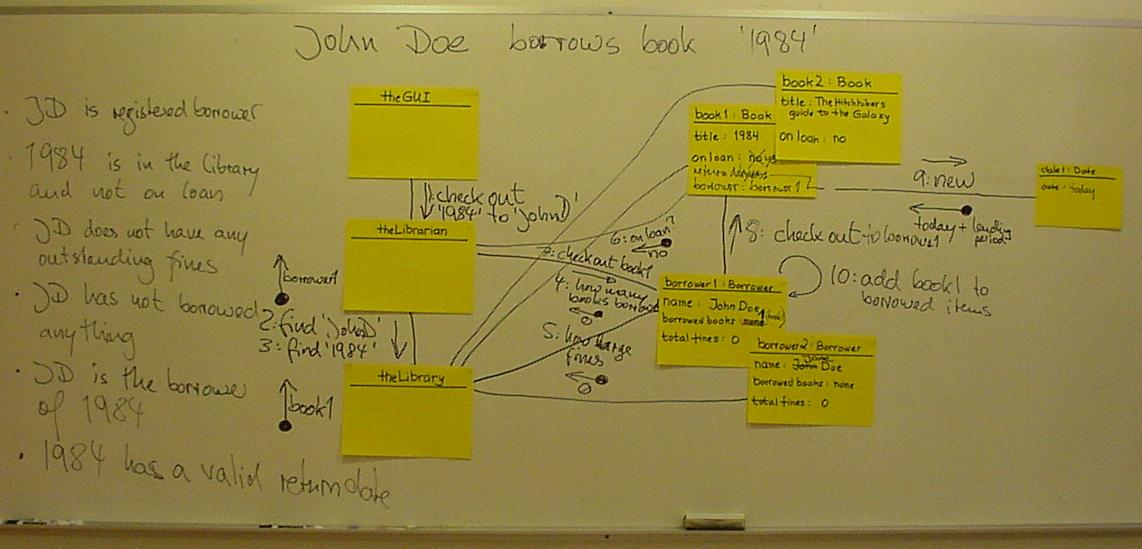
\includegraphics[width=\textwidth]{example_picture} % you can use other formats too
   \caption{Another figure; this time from a JPG file.\label{fig:picture}}
\end{figure}

As mentioned, \LaTeX\ automatically moves floats to a ``good'' place, normally near
the place where the environment is found in the source file. Thus, as a rule of thumb,
the environment should be placed near the position where you refer to the table or figure
for the first time, even though it could in principle be added anywhere. Many authors
have quite distinct ideas about the optimal placement of a float in the compiled paper.
In fact, this placement can be affected by optional arguments to the floating
environments. \emph{Please do not make use of these possibilities!} One reason is that
the automatic placement defined by the style (in this case the LNCS style) is intended
to create a uniform ``look and feel'' which is destroyed by manual formatting. The other,
more important reason is that including the paper in the proceedings may lead to
slight changes in, e.g., page breaks. In such cases, manually placed tables and figures
can end up in very unsatisfactory places.

\section{Further Remarks}

Below, some more hints are collected that you should use when preparing your full paper
and the final version. In fact, you should follows these recommendations from the very
beginning, because it saves time to do it right from the start.

\subsection{More about Manual Formatting}
In principle, \LaTeX\ gives you\\
\hspace*{-2em}all p\raisebox{1pt}os\hspace{.2ex}si\raisebox{-.5ex}bi\hspace{-.5ex}li\rotatebox{180}tie\scalebox{5}[1]s in the world\\[.5ex]
\hspace*{2em}for manual typesetting\\[-1.5ex]
\hspace*{2cm} in all kinds of weird ways.\footnote{In fact, this statement
is literally true to the extent possible, because \LaTeX\ 
is Turing complete. Thus, every computable layout can be implemented in \LaTeX.} Please refrain
from using them, including manual
linebreaks (except in places where these are intended to be used, e.g., to
end a row in a \texttt{tabular} environment), \texttt{\string\noindent}, \texttt{\string\bigskip},
and the like, the reasons basically being the same as those for avoiding manual placement
of floats. Of course, you should even more strictly refrain from changing general layout parameters such
as \texttt{\string\parskip} and \texttt{\string\parindent}.

\subsection{Referring to Internet Resources}

People use different ways to refer to homepages, forums, and other types of Internet resources.
Some treat them as ordinary references and include them in their reference section, such
as~\cite{bluej}. However, since such material is quite different in character from real scientific
publications, a cleaner solution is to use the reference section only for ordinary references and
add footnotes to point to other material, e.g., when writing about BlueJ\footnote{\url{http://www.buej.org},
BlueJ tool homepage, accessed 2005-01-12}. Note that, nowadays, even scientific publications
sometimes lack a printed version and are available only electronically (such as,
e.g.,~\cite{Corradini-Drewes:11}). Of course, such publications
should nevertheless be included in the list of references. The important point is not whether
material is printed or not, but which role it plays.

\section{A Checklist for the Full Version}

When your full version is complete and ready for submission, please spend a few minutes to
check the following, using the search facility of your favorite editor:
\begin{itemize}
\item You have taken care of the adjustments necessary to be made when switching from
the outline and annotated bibliography to the actual style of the article. In particular,
this means that you do not use the \texttt{oribibl} option in the \texttt{\string\documentclass}
command, the BIBTeX style used is \texttt{splncs}, and the command \texttt{\string\nocite\{*\}}
has been removed or commented out.
\item Words in the title of the paper and in section and subsection headings are correctly
capitalized.
\item Spaces in front of \texttt{\string\ref}, \texttt{\string\pageref}, and \texttt{\string\cite}
are nonbreaking. (Also, make sure that there actually \emph{are} spaces in front of them!) Again,
note that there might be small changes in the layout when the proceedings are produced. Therefore,
it is not guaranteed that all line breaks will stay the same.
\item Check the list of references carefully. If something is strange, correct
the corresponding record in your BIBTeX file. Note that names of authors and editors
in the \texttt{author} and \texttt{editor} fields should preferably be formatted according to
\texttt{last name(s), first name(s)}, and multiple authors/editors must be separated by the
keyword \texttt{and}. In titles, abbreviations such as UML should be enclosed in curly brackets
(i.e., \texttt{\{UML\}}) to prevent BIBTeX from turning them into lowercase.
\item Check whether you use ordinary double quotation marks \texttt" in your \LaTeX\ source. If
so, replace each by two single quotation marks: \verb;``; on the left and \verb;''; on the right,
thus turning, e.g., "fishy" into ``fishy''.
\item Typeset URLs by means of the command \texttt{\string\url}.
\end{itemize}

%%%%% BEGIN OF 3rd ADJUSTMENTS SECTION %%%%%
% For the outline and annotated bibliography (deliverable 2)
% you must use the following two commands:
%
\nocite{*}  % Includes ALL entries from the .bib-file, even if they are
            % not '\cite{}'-ed in the text above
\bibliographystyle{plain-annote}
%
%For the full and final paper (deliverables 3 and 4a/b)
% use ONLY the following commands (i.e. put the commands above into
% comments and uncomment the command below):
%
% \bibliographystyle{splncs}
%
%%%%% END OF ADJUSTMENTS SECTION %%%%%

\bibliography{demo}

\end{document}
